\section{Kriteriji za klasifikacijo spletnih portalov}
\label{sec:kriteriji_za_klasifikacijo_spletnih_portalov}

Spletni portali za učenje programiranja imajo različne značilnosti in
zmožnosti. V poglavju bomo razdelali posamezne kriterije, s katerimi
bomo klasificirali in ovrednotili posamezne spletne portale.

\subsection{Vrsta vsebine}
\label{sec:Razvrstitev_spletnih_portalov}

Po prvem pregledu in iskanju spletnih portalov lahko ugotovimo, da
spletni portali za učenje programiranja ponujajo najrazličnejše vrste
vsebin in njihove kombinacije, kot je na primer, \textbf{tekstovni
  vodič in spletna aplikacija za programiranje}. V posebno kategorijo
bomo uvrstili tudi spletne portale, ki ponujajo \textbf{spletne igre},
ki učijo programiranje. Različne vrste spletnih portalov, ki jih lahko
obravnavamo, so naslednje:

\begin{itemize}
\tightlist
\item \textbf{tekstovni vodiči},
\item \textbf{video vodič},
\item \textbf{spletna aplikacija za programiranje}, kot smo jo
  definirali v poglavju \ref{sec:značilnosti_spup},
\item \textbf{spletne igre},
\item \textbf{kombinacija} vrst vsebin, ki jih lahko še razdelimo na:
  \begin{itemize}
    \tightlist
  \item \textbf{najosnovnejša kombinacija} (\emph{tekstovni vodič + preizkus kode});
  \item \textbf{napredna kombinacija} (\emph{različne vrste vodičev +
      spletna aplikacija za programiranje}), ki tvorijo \textbf{vadnice}.
  \end{itemize}
\end{itemize}

V tej diplomskem delu se ne bomo podrobno ukvarjali s tem, katera izmed vrst
vsebin predstavlja boljše zmožnosti za prenos znanja. Vsaka ima svoje
prednosti in slabosti, zato bomo za vsako izpostavili le bistvene
pozitivne značilnosti in tudi slabosti. Zanimale nas bodo predvsem
tiste \textbf{kombinirane} vrste vsebin, ki bodo predstavljale čim bolj
celovit spletni portal za učenje programiranja, kot smo ga definirali
v poglavju \ref{sec:značilnosti_spup}.

\subsubsection{Tekstovni vodiči}

Spletni vodiči veljajo za starejše metode podajanja znanja na
spletu. Za njih je značilno, da uporabnika vodijo \textbf{po korakih}
do nekega določenega cilja, kako nekaj narediti, ali specifičnega
znanja. Besedilo, ki podaja znanje, je opremljeno s
\textbf{primeri}. \cite{wiki:tutorials}

Značilni predstavnik takih vodičev je spletna stran
\url{https://docs.python.org}, na kateri najdemo vso dokumentacijo
programskega jezika \textbf{Python}. Na strani najdemo tudi vodiča z
naslovom \emph{\href{https://docs.python.org/3/tutorial/index.html}{The
  Python Tutorial}} \cite{web:TPythonTut}.

\begin{figure}[h!]
  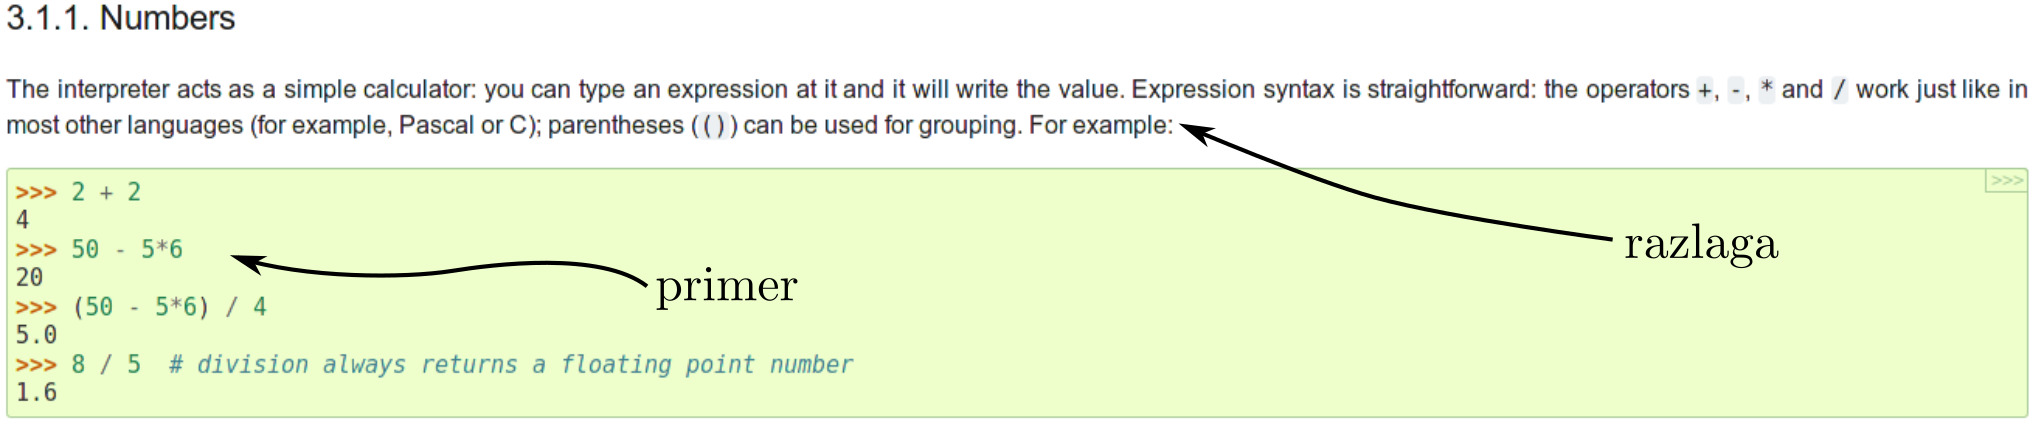
\includegraphics [width=1\linewidth, keepaspectratio =
  1] {./images/sc_web/tPyTut_01.jpg}
    %\def\svgwidth{\columnwidth}
    %\input{./pdf_tex/tPyTut_01.pdf_tex}
      \caption{Zaslonski posnetek poglavja z vodiča
      \emph{\href{https://docs.python.org/3/tutorial/index.html}{The
          Python Tutorial}} s primerom \cite{web:TPythonTut}.}
    \label{fig:scr:web:tPyTut}
\end{figure}

Spletne vodiče pri pouku uporabljamo na podoben način, kot bi vodiča,
napisanega na učnem listu z \textbf{metodo dela s tekstom}. Sicer je
pomembno, da učenci usvojijo uporabo spletnih vodičev, vendar so
spletni vodiči marsikdaj prezahtevni za uporabo, sploh na osnovnošolskem nivoju, z vso tehnično dokumentacijo. Negativna stran spletnih
vodičev je še ta, da ne moramo neposredno s spletne strani preizkušati
primerov programske kode, kar je slabo tudi z motivacijskega vidika.

\subsubsection{Video vodiči}
\label{sec:video_vodici}

Z razmahom video vsebin na spletu so marsikateri spletni vodič
dopolnili oz. jih zamenjali video vodiči. Popularno je postalo
zajemanje oz. \textbf{snemanje lastnega namizja}. Video vodiče najdemo
za številna področja, od uporabe določene programske opreme in vse do
programiranja. Ena izmed prednosti video vodičev je
ta, da ti omogočajo nazornejši prikaz nekega postopka po
korakih. Preden sami opravimo nek postopek, lahko v video posnetku
opazujemo vsak korak, potek miške in poleg tega poslušamo razlago, če
je ta vključena. Številne študije kažejo, da je učenje z multimedijo,
torej kombinacijo zvoka in slike,  učinkovitejše kot samo poslušanje ali
branje teksta \cite{web:multimediaL}. V razredu je uporaba video
vodičev lahko koristna pri samostojnem in domačem delu. Uporaba
video vodičev ima tudi slabe strani, v njih lahko predstavimo dosti
manj vsebine in iskanje po vsebini v video ni preprosto, kot je to pri
tekstu.

Eden izmed spletnih portalov, ki je specializiran za podajanje znanja
z video vodiči, je \emph{\href{https://www.udemy.com}{Udemy}}
\cite{web:udemy}. Na njem lahko vsakdo  postane učitelj in pripravi
učne ure z različnih področij, ne samo z računalniške
znanosti. Nekateri sklopi učnih ur so v celoti brezplačni, kljub temu
je večina plačljivih.

\begin{figure}[h!]
    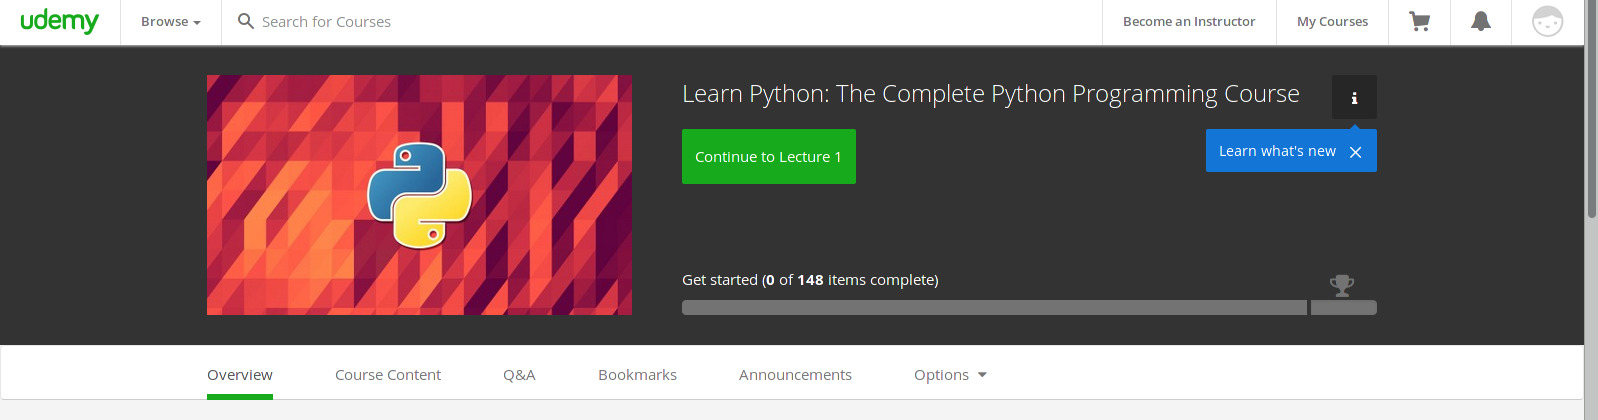
\includegraphics [width=1\linewidth, keepaspectratio =
    1] {./images/sc_web/udemy_01.jpg}
    \caption{Uvodna stran enega izmed video vodičev za učenje Pythona
      \cite{web:udemy}.}
    \label{fig:scr:web:udemy}
\end{figure}

\subsubsection{Spletna aplikacija za programiranje}
\label{sec:spletna_app_programiranje}

Nekatere spletne strani ponujajo le spletno aplikacijo za
programiranje, kot smo jo povzeli v poglavju
\ref{sec:značilnosti_spup}. Taki spletni portali ne ponujajo vsebine,
ponujajo le aplikacijo, ki jo uporabimo kot \textbf{orodje}. Ali pa
ponujajo le toliko vsebine, kot je potrebno, da se uporabnik nauči
uporabljati spletno aplikacijo. Kljub temu da nas zanimajo celoviti
spletni portali, ki ponujajo tudi vsebino, nas bodo podrobneje
zanimala tudi orodja, saj so ta ključna za nekatere prednosti, ki jih
ponujajo spletni portali za učenje programiranja. Predstavnik takega
orodja je \emph{\href{http://pythonfiddle.com/}{Python Fiddle}}
\cite{web:pythonfiddle}. Omogoča osnovni urejevalnik besedila (slika)
z barvanjem programske kode, s predlogami za samodokončanja izpisa
vgrajenih funkcij. Uvozimo lahko datoteke in jih delimo. Zaganjamo
napisane programe, izhodni podatki se izpišejo v konzoli.

\begin{figure}[h!]
    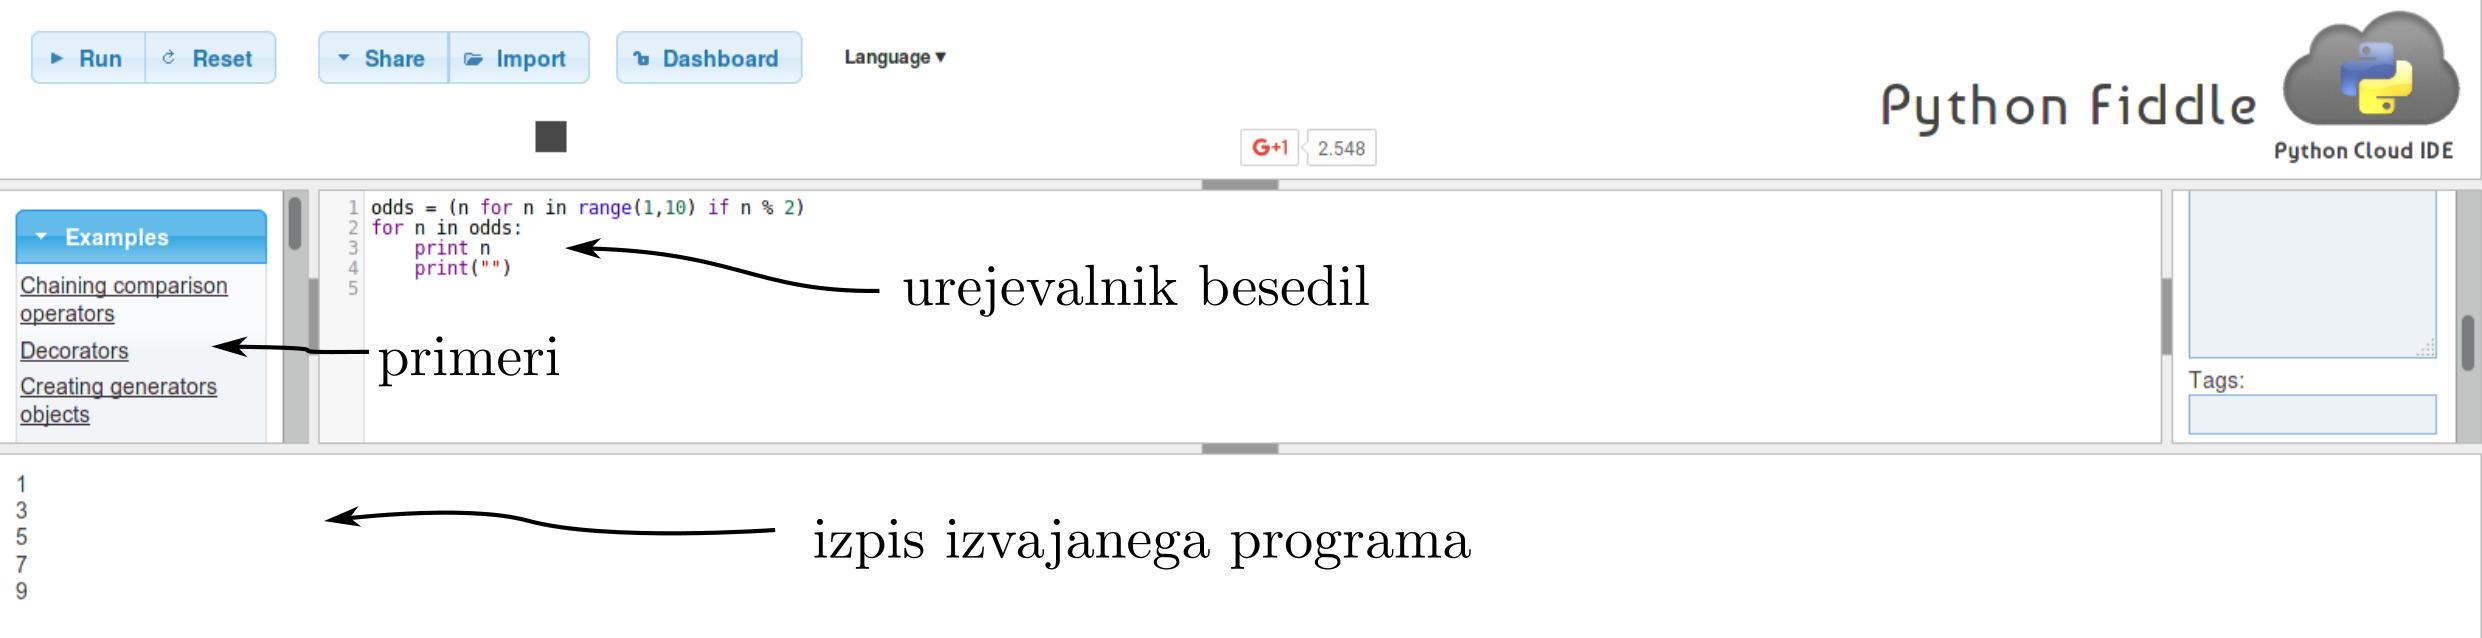
\includegraphics [width=1\linewidth, keepaspectratio =
    1] {./images/sc_web/PythonFiddle_01.jpg}
    \caption{Zaslonska slika spletne aplikacije za programiranje
      \emph{\href{http://pythonfiddle.com/}{Python Foddle}}
      \cite{web:pythonfiddle}.}
    \label{fig:scr:web:PyFiddle}
\end{figure}

Spletne tehnologije so danes zelo napredovale in že nekaj let se
aplikacije in podatki selijo v \textbf{oblak}. Te aplikacije in
podatki so dostopni kjerkoli. V \textbf{oblaku} se razvijajo
številna profesionalna okolja \textbf{IRO}, ki omogočajo delo na
večjih projektih in ponujajo napredne funkcije IRO, ki smo jih drugače
lahko imeli le z namiznimi aplikacijami. Navedimo dva primera:
\emph{\href{https://codenvy.com/}{Codenvy}} \cite{web:codeenvy} in
\emph{\href{https://c9.io/}{Cloud9}}\cite{web:cloud9}. Oba ponujata
profesionalni IRO v oblaku. Za uporabo v šoli sta ti dve okolji preveč
zahtevni in jih ni smiselno uporabljati pri poučevanju novincev. S
tem jim otežimo učenje programiranja, saj potrebujejo čas, da
spoznajo in se naučijo uporabljati IRO.

\subsubsection{Spletne igre}
\label{sec:spletne_igre}

Na spletu obstajajo številni spletni portali, ki učijo in spodbujajo k
učenju programiranja z igram podobnimi vsebinami. Vsebina je
razdeljena na stopnje. Igralci napredujejo iz stopnje v stopnjo in pri
tem nabirajo izkušnje, nove veščine in dosežke. Za igranje igre ne
upravljamo gibanja lika v igri s tipkovnico in miško, temveč pišemo
programsko kodo, ki upravlja njihovo početje. Takšni spletni portali
dajejo zelo dobro motivacijsko osnovo, saj se novinci spoznajo na
osnovne principe igranja iger. Primer spletnega portala je
\emph{\href{http://fightcodegame.com/}{Fightcode}}
\cite{web:fightcode} (slika \ref{fig:fightcode}). Igralci programirajo robota v programskem jeziku
JavaScript. Vsak izmed igralcev lahko izzove drugega igralca v boj med
roboti. Za vsako zmago se igralec pomika navzgor po lestvici
najboljših robotov.

\begin{figure}[h!]
    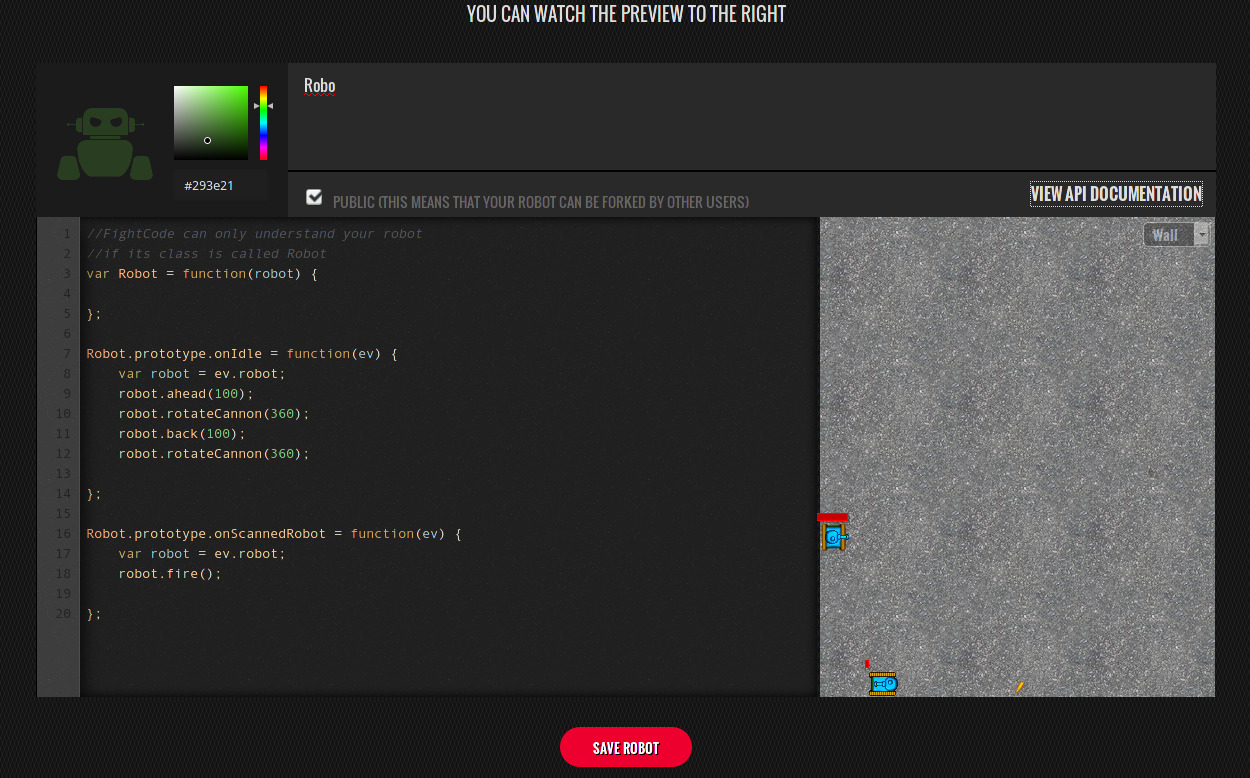
\includegraphics [width=1\linewidth, keepaspectratio =
    1] {./images/sc_web/fightRobot_01.jpg}
    \caption{Zaslonska slika spletne strani
      {\href{http://fightcodegame.com/}{Fightcode}}
      \cite{web:fightcode}.}
    \label{fig:fightcode}
\end{figure}

V nadaljevanju si bomo še podrobneje ogledali značilnosti nekaterih drugih
spletnih iger, ki učijo programirati.

\subsubsection{Kombinirane vrste vsebin}
\label{sec:kombinirane_vrste_vsebin}

V prejšnjih poglavjih smo opisali \textbf{osnovne vrste} spletnih
portalov. Zanimale nas bodo predvsem \textbf{kombinirane vrste}, ki so
sestavljene iz osnovnih. Na spletu najdemo številne kombinacije
spletnih portalov. \textbf{Osnovno kombinirano vsebino} predstavljajo
spletni portali, kot je
\emph{\href{http://www.w3schools.com/}{w3School}} (slika
\ref{fig:scr:web:w3school}) \cite{web:w3school}. Sestavljeni so iz
\textbf{tekstovnih vodičev} in \textbf{najosnovnejšega preizkusa
  programske kode}. Vsak primer v vodiču je opremljen s primerom,
ki ga lahko zaženemo in preizkusimo. Za izvajanje primera
pritisnemo na gumb \textbf{Preizkusi!  (\emph{ang. Try it!})}
Programsko kodo primera lahko tudi spreminjamo in jo ponovno izvajamo.

\begin{figure}[h!]
    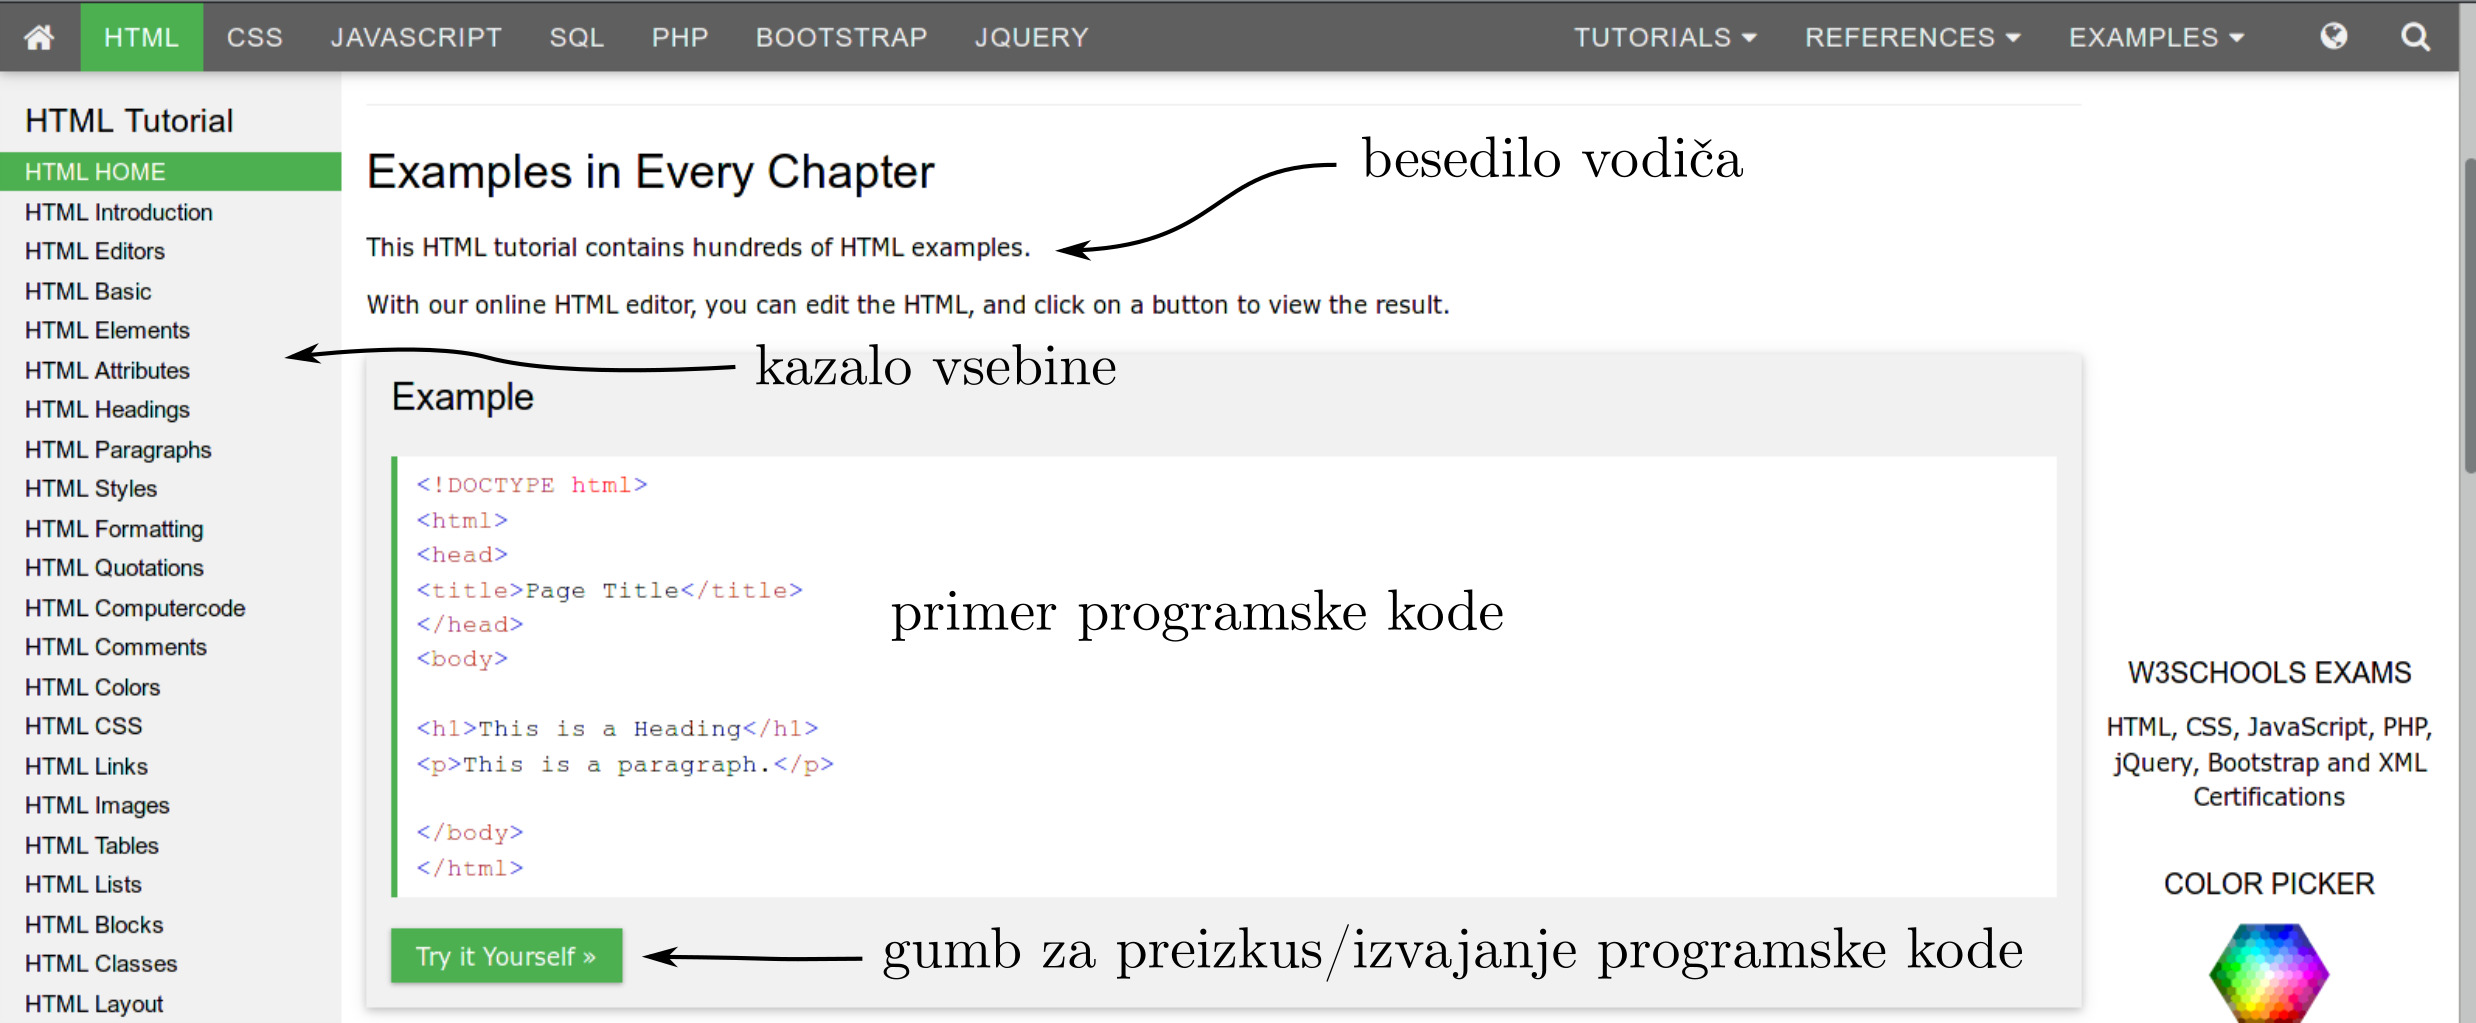
\includegraphics [width=1\linewidth, keepaspectratio =
    1] {./images/sc_web/w3school.jpg}
    \caption{Zaslonska slika spletne strai
      \emph{\href{http://www.w3schools.com/}{w3School}}
      \cite{web:w3school} v poglavju HTML.}
    \label{fig:scr:web:w3school}
\end{figure}

\textbf{Napredno kombinirano vsebino} predstavljajo spletni portali,
ki so sestavljeni iz \textbf{tekstovnega vodiča in/ali video vodičev ter
  spletne aplikacije za programiranje}. Omenimo naslednjega
predstavnika \emph{\href{https://www.codeschool.com/}{Codeschool}}
\cite{web:codeschool}. Taki napredni kombinirani vsebini pravimo \textbf{vadnica}. V njej je navadno podana razlaga, zastavljen
problem oz. naloga, ki ga rešujemo v urejevalniku besedil. V vadnici
imamo navadno še  preverjanje rešitev, torej sintaktično preverjanje
pravilnosti napisane programske kode, ter pravilnost rešitve naloge.

\begin{figure}[h!]
    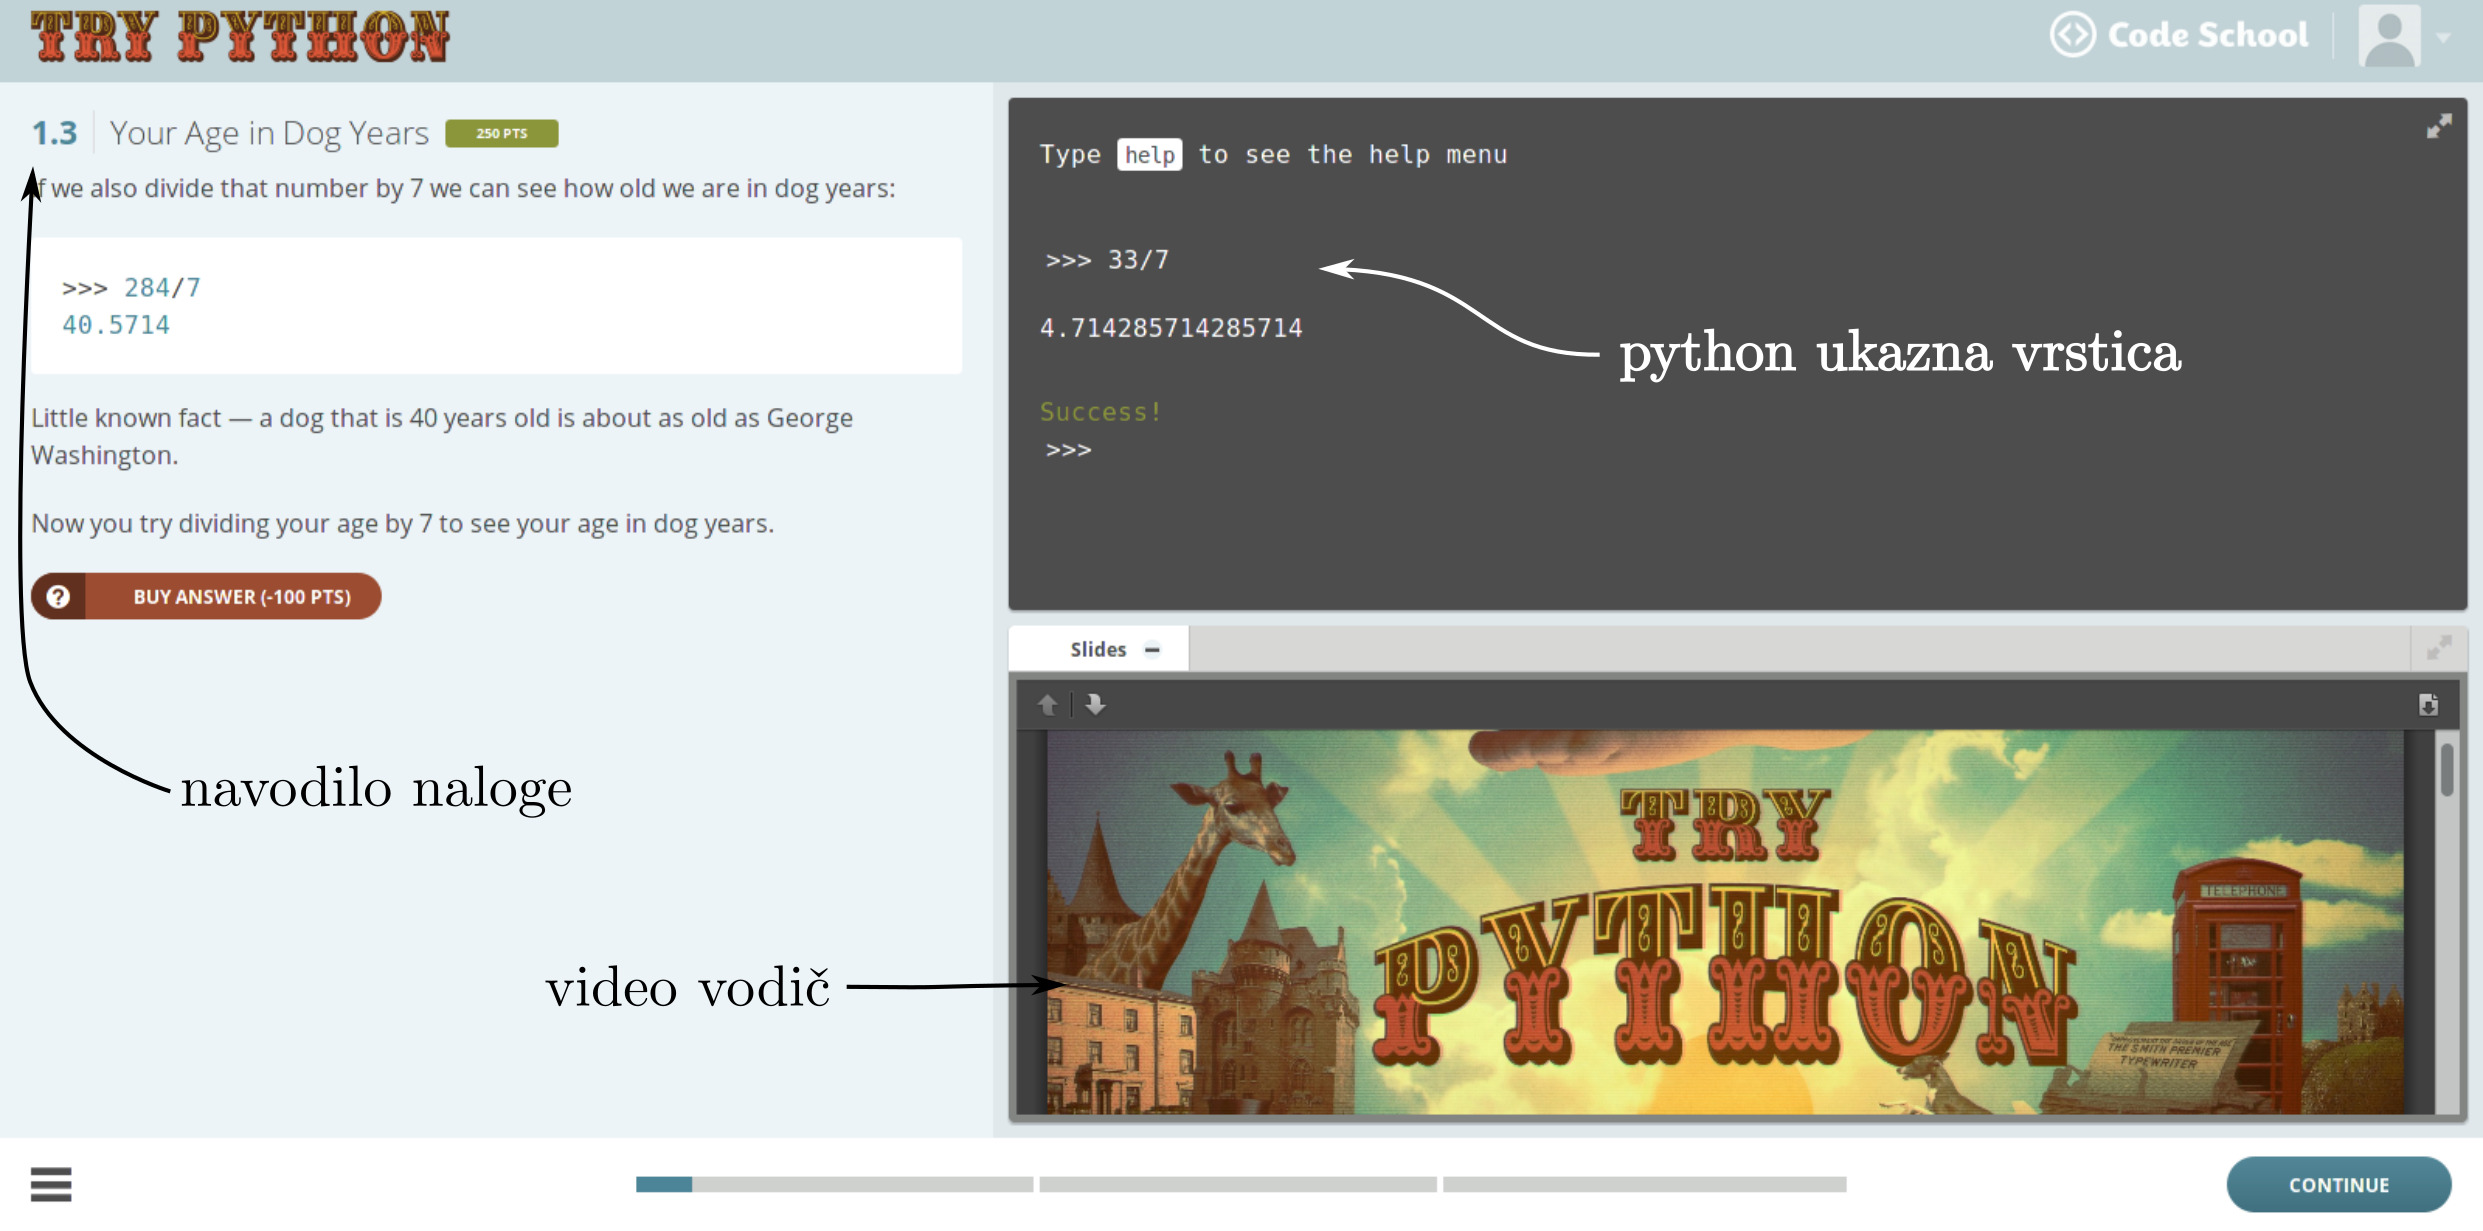
\includegraphics [width=1\linewidth, keepaspectratio =
    1] {./images/sc_web/codeschool_01.jpg}
    \caption{Zaslonska slika spletne strani
      \emph{\href{https://www.codeschool.com/}{Codeschool}}
      \cite{web:codeschool}.}
    \label{fig:scr:web:codeschool}
\end{figure}

Različne kombinirane vsebine imajo različne zmožnosti, ki jih bomo
spoznali na konkretnem primeru v podrobnem pregledu.

\subsection{Jezik spletnega portala}
\label{sec:jezik_spletnega_portala}

Ugotovimo lahko, da večina spletnih portalov uporablja
\textbf{angleščino} kot primarni jezik. Nekateri ponujajo tudi druge
jezike, vendar je \textbf{slovenščina} zaradi majhnosti le malokrat
zajeta, razen v redkih primerih. Angleščina je glavni jezik spleta in
računalniške znanosti, zato je pomembno, da učenci oz. dijaki spoznajo
tudi angleške izraze in jih povežejo s pravilnimi
slovenskimi. Kljub temu da je učenje v slovenskem jeziku predpisano,
lahko vsako učno uro z uporabo spletnih portalov za učenje
programiranja medpredmetno povežemo z angleščino. Zanimalo nas bo,
kateri jezik uporabljajo spletni portali: \textbf{angleščina (da/ne),
  slovenščina (da/ne), drugi (da/ne)}.

\subsection{Ponujena znanja}
\label{sec:vsebina_problemsk_pristop}

Spletne strani za učenje programiranja navadno ponujajo znanja oz.
veščine programiranja z določenim programskim jezikom. Nekatera svojo
ponudbo širijo tako, da ponujajo številne druge projekte, ki
združujejo prej naučeno znanje. Na primer izdelava
\textbf{interaktivne spletne strani}. Za posamezen spletni portal nas
bo zanimalo, ali ponuja samo:

\begin{itemize}
  \tightlist
\item \textbf{znanja/veščine programiranja} oz. učenje določenega
  programskega jezika,
\item \textbf{znanje algoritmov} ali tudi
\item \textbf{druga projektna znanja/veščine} (npr. izdelava spletne
  strani).
\end{itemize}

% Zanimajo nas osnovna načela. -> Razdelaj na načela

\subsection{Programski jeziki}
\label{sec:_zanaja_programski_jeziki}

Zanimalo nas bo, katere programske jezike ponuja nek spletni
portal. Najpogostejše programske jezike smo opisali v poglavju
\ref{sec:programski_jeziki}, v prvi vrsti nas bodo zanimali spletni
portali, ki ponujajo najpopularnejše programske jezike in tiste, ki
se v izobraževanju uporabljajo pri nas. Prednost bodo imeli tisti,
ki ponujajo Python. Večina takšnih spletnih portalov ponuja več
programskih jezikov.

\subsection{Težavnostna stopnja}
\label{sec:težavnostna_stopnja}

Vsak spletni portal je namenjen svojemu občinstvu, zato se razlikujejo tudi po težavnostni stopnji, čeprav govorimo o novincih. Glavna
težavnostna razdelitev bo na \textbf{osnovo} in \textbf{srednjo
  šolo}. Po potrebi bomo podrobneje razdelili že osnovno šolo, ki je
razdeljena na triletja. Večina spletnih portalov izhaja iz Združenih
držav Amerike, zato smo povzeli njihove stopnje šolanja
(\ref{tab:primerjava_šolski}), saj nekatere strani uporabljajo
\textbf{K-12} formulacijo za definicijo težavnosti oz. prilagoditev
učnemu načrtu. V podrobnem pregledu bomo ocenili, kateri težavnostni
stopnji ustreza spletni portal.

\begin{table}[!h]
\caption{Primerjava starosti in stopnje šolanja šolskega sistema v ZDA
  in Sloveniji \cite{wiki:k12}.}
\label{tab:primerjava_šolski}
\begin{tabular}{
  | p{0.33\linewidth-2\tabcolsep} |
  p{0.33\linewidth-2\tabcolsep} |
  p{0.33\linewidth-2\tabcolsep} |  }
\hline
  \rowcolor{sbase01!100}
  \textbf{Leta} & \textbf{ZDA K-12 naziv} & \textbf{SI Primerjava} \\
        \hline
      6-10    & \emph{Elementary school} & \textbf{1. in 2. triletje
                                             OŠ}\\
        \hline
      10-14    & \emph{Middle school} & \textbf{3. triletje OŠ} \\
        \hline
  10-14    & \emph{High school} & \textbf{Srednja šola} \\
  \hline
\end{tabular}
\end{table}

%Razdelaj načele problemski pristop. postopnosti in sistematičnosti.
\subsection{Upoštevanje učnih načel}
\label{sec:upoštevanje_načel}

Za uspešno delo in uporabo SPUP v razredu je dobro, da vsebine, ki jih
najdemo na spletu, sledijo že v samem jedru nekaterim \textbf{načelom}, ki jih
upoštevamo tudi drugače pri pouku.

\begin{description}
\item[Problemski pristop (Da/Ne)], zanima nas ali spletni portali, ki
  ponujajo vsebino, uporabljajo problemsko zasnovane naloge, torej imajo
  v začetku obravnavanja snovi podano oz. predstavljeno, kateri problem
  bomo znali na koncu neke vadnice rešiti. Čeprav je vsebina
  računalniške znanosti in programiranja že po naravi problemsko
  zasnovana, marsikdaj ni najbolje predstavljeno, za kaj je neka stvar
  dobra.
\item[Načelo sistematičnosti (Da/Ne)], lahko potrdimo za tiste
  spletne portale, kjer so posamezni vsebinski sklopi povezani v nekem
  logičnem zaporedju. Kot smo že ugotovili pri pregledu spletnih
  portalov na univerzah, je pomembno, da novinci spoznajo nekatere
  koncepte prej kot druge. Tiste spletne portale, ki bodo imeli neko
  rdečo nit v povezavi vsebine, bomo potrdili kot take.
\item[Načelo postopnosti (Da/Ne)], pripišemo lahko spletnemu portalu,
  ki podaja snov v posameznem vsebinskem sklopu tako, da bo razlago
  in program nadgrajeval postopoma in se težavnost stopnjuje.
\end{description}

\subsection{Uporaba ocenjevanja dosežkov, značilnih za igre}
\label{sec:uporaba_dosežkov}

%ToDo: Slovenski izraz za Gamification.
V izobraževanju se uveljavlja trend ocenjevanja napredka in dosežkov,
ki je tipičen za video igre. To metodo ocenjevanje so poimenovali
\emph{ang. Gamification}. Vsako snov ali nalogo, ki je v osnovi toga,
popestrimo z načinom ocenjevanja tako, da vsako nalogo predstavimo z
različnimi izzivi. Vsaki nalogi oz. izzivu sledijo različne nagrade,
ki jih učenci zbirajo in jim pravimo dosežki \cite{web:edublogger}.

Dosežki v video igrah so prisotni že vrsto let. Dosežki se razlikujejo
po kompleksnosti, vse od zmagoslavne glasbe ob končani stopnji ali
igri pa vse do kompleksnega sistema dosežkov z zbiranjem
značk. Značko igralec dobi, ko na primer zbere dovolj predmetov ali
razišče določen odstotek ozemlja. Poznamo več načinov nagrajevanja
dosežkov. Kot smo že omenili, lahko dosežke predstavimo kot
\textbf{značke} ali za posamezne izzive pripravimo sistem točkovanja. Z zbranih točk se lahko sestavijo \textbf{lestvice
  ali uvrstitve}. V razredu  morajo biti slednje skrbno načrtovane, da
ne pride do prevelikih razlik med učenci, kjer bi se eni lahko
počutili nadrejeni in drugi podrejeni.

Zanimalo nas bo, ali spletne portali, ki učijo programiranja,
uporabljajo kakršen koli sistem ocenjevanja dosežkov, saj za tiste, ki
ga uporabljajo, lahko rečemo, da imajo dodaten motivacijski
faktor. Zapisali bomo \textbf{uporabo dosežkov (da/ne)} in tipe
\textbf{značke, lestvice, zbiranje točk za izkušnje, napredovanja  \dots}

\subsection{Dodajanje lastnih vsebin}
\label{sec:dodajanje_vsebin}

Nekateri spletni portali omogočajo, da pripravimo lastne vsebine, ki
jih potem delimo. Navadno je \textbf{spletna aplikacija za
  programiranje} ali \textbf{vadnica} razširjena tako, da omogoča
sestavljanje programskih nalog. Večina teh je taka, da pripravimo
\textbf{spremno besedilo, začetni program ali ogrodje programa, končno
  različico in pomoč ali namig}. Lahko so dodani tudi \textbf{testni
  vhodni in izhodni podatki}. S podatki, ki smo jih vnesli, imamo
avtomatizirano nalogo, ki jo lahko posredujemo oz. delimo z
novincem. Zanimalo nas bo, ali kateri spletni portal omogoča to
zmožnost, torej \textbf{dodajanje lastnih vsebin (da/ne)}.

\subsection{Upravljanje razreda}
\label{sec:upravljanje_razreda}

Zmožnost upravljanja razreda je velika prednost in olajša administrativno delo
 razreda za mentorja. Osnovni način delovanja je
naslednji. Mentor ustvari razred ali predmet podobno, kot je to možno
pri sistemih spletnih učilnic, kot je
\emph{\href{https://moodle.org/}{moodle}} \cite{web:moodle_site}, in v
učilnico povabi učence. Učitelj s spletne učilnice \textbf{spremlja
  napredek} in \textbf{dosežke posameznega učenca}. Pri nekaterih
portalih je \textbf{omogočena komunikacija} med mentorjem in
novincem. Spletni portali spremljanje učencev navadno ponujajo kot
plačljivo storitve za šole, kar navadno ni najbolj poceni. Zanimalo
nas bo, ali spletni portal ponuja \textbf{upravljanje razreda (da/ne)}
in ali je ta storitev \textbf{plačljiva ali brezplačna}.

\subsection{Dostop do gradiv}
\label{sec:dostop_do_gradiv}

Veliko vsebin na spletu je brezplačnih in jih pri pouku lahko
uporabimo. Mnogo vsebin je tudi plačljivih. Spletni portali, ki imajo
plačljive vsebine, uporabljajo navadno model \textbf{plačevanja
  naročnine} za dostop do vsebin. Uporabnik mora na \textbf{letni ali
  mesečni} ravni odšteti različne zneske. Nekateri izmed portalov, kot
je \emph{Codeacademy}, imajo plačljive le nekatere zahtevnejše vsebine
in storitve. Drugi portali imajo vso vsebino
plačljivo. Obstaja tudi vrsta portalov, kot je \emph{Udemy}, kjer je
potrebno plačati za posamezen učni sklop ali temo.  Plačljivost
dostopa do gradiv lahko razvrstimo na naslednji način, tako da je
dostop:

\begin{itemize}
  \tightlist
\item brezplačen,
\item polplačljiv \emph{(nekatere so brezplačne, druge plačljive)},
\item popolnoma plačljive vsebine.
\end{itemize}

%%Dodaj nekaj (3) spletnih portalov, ki so popolnoma plačljivi!

%%% Local Variables:
%%% mode: latex
%%% TeX-master: "../diploma"
%%% End:
